\section{Hadoop MapReduce}
\label{sec:hadoop}

Como parte del proyecto, el grupo ejecutó tres programas incluidos en \texttt{hadoop-mapreduce-examples.jar} sobre el clúster de Dataproc, usando HDFS como sistema de archivos distribuido, tal como exige el enunciado. Se eligieron \texttt{wordmean}, \texttt{wordmedian} y \texttt{secondarysort}, cualquier programa del jar está permitido salvo \texttt{wordcount} y \texttt{grep}, por tener sintaxis simple (\texttt{<input> <output>}, sin argumentos ambiguos) y por poder aplicarse directamente sobre columnas reales del dataset.

\subsection{Preparación de los inputs}

A partir del CSV original se extrajeron dos archivos de texto plano:

\begin{itemize}
    \item \texttt{descriptions.txt}, una descripción de producto (columna \texttt{Description}) por línea.
    \item \texttt{customer\_quantity.txt}, pares de valores \texttt{CustomerID} y \texttt{Quantity} separados por un espacio, uno por línea.
\end{itemize}

Ambos se subieron a \texttt{gs://<bucket>/input/} y de ahí se copiaron a HDFS (\texttt{/retail/}) antes de correr los jobs.

\subsection{Los tres programas}

\begin{table}[H]
\centering
\begin{tabular}{lll}
\toprule
\textbf{Programa} & \textbf{Objetivo} & \textbf{Input} \\
\midrule
\texttt{wordmean} & Largo promedio de palabra & \texttt{descriptions.txt} \\
\texttt{wordmedian} & Mediana del largo de palabra & \texttt{descriptions.txt} \\
\texttt{secondarysort} & Agrupar por clave y ordenar por una segunda & \texttt{customer\_quantity.txt} \\
\bottomrule
\end{tabular}
\caption{Programas de \texttt{hadoop-mapreduce-examples.jar} utilizados}
\end{table}

Se eligieron estos tres programas porque cada uno mide algo distinto y útil sobre el catálogo. \texttt{wordmean} y \texttt{wordmedian} miden el largo de las descripciones de producto, con un catálogo de más de 5{,}000 productos distintos, saber qué tan largas son típicamente las descripciones importa para dimensionar índices de búsqueda o reglas de truncado en una interfaz. \texttt{secondarysort} agrupa todas las compras de cada cliente y las ordena internamente por cantidad, lo que deja ver, cliente por cliente, si su patrón de compra es de pedidos chicos y sueltos o de pedidos grandes y repetidos (ver la Sección \ref{sec:hadoop-resultados}). Este último programa demuestra además el patrón de \emph{secondary sort} de MapReduce: agrupar por una clave mientras se ordena por una segunda dentro de cada grupo, algo que requiere una lógica de partición/orden compuesta y no es trivial de lograr con un \texttt{reduce} simple.

\subsection{Comando ejecutado}

Cada job se envió mediante \texttt{gcloud dataproc jobs submit hadoop}, la forma nativa de correr jobs en Dataproc, que hace \emph{polling} del estado del job vía la API sin depender de una conexión SSH persistente al clúster. El comando exacto ejecutado para cada uno de los tres programas fue:

\begin{verbatim}
gcloud dataproc jobs submit hadoop \
  --cluster=dataproc-cluster --region=southamerica-west1 \
  --jar=file:///usr/lib/hadoop-mapreduce/hadoop-mapreduce-examples.jar \
  -- <programa> <input_hdfs> <output_hdfs>
\end{verbatim}

donde los tres parámetros toman los siguientes valores según el programa que se esté ejecutando:

\begin{table}[H]
\centering
\small
\begin{tabular}{lp{9cm}}
\toprule
\textbf{Parámetro} & \textbf{Valor} \\
\midrule
\texttt{<programa>} & \texttt{wordmean}, \texttt{wordmedian} o \texttt{secondarysort} \\
\texttt{<input\_hdfs>} & \url{/retail/descriptions.txt} o \url{/retail/customer_quantity.txt}, según corresponda \\
\texttt{<output\_hdfs>} & \texttt{/retail/<programa>} \\
\bottomrule
\end{tabular}
\caption{Parámetros del comando de envío de jobs Hadoop}
\end{table}

El resultado de cada job (las particiones \texttt{part-r-00000}, \texttt{part-r-00001}, \ldots generadas por los \emph{reducers}) queda almacenado en HDFS, dentro del clúster, tal como exige el enunciado. Recién después, para poder explorarlo y conservarlo más allá de la vida del clúster, se juntan esas particiones en un solo archivo y se copian a Cloud Storage:

\begin{verbatim}
hadoop fs -getmerge /retail/<programa> /tmp/<programa>.txt
gsutil cp /tmp/<programa>.txt gs://<bucket>/output/<programa>.txt
\end{verbatim}

\subsection{Evidencia y resultados}
\label{sec:hadoop-resultados}

La Figura \ref{fig:dataproc-jobs} muestra los tres jobs completados exitosamente sobre el clúster.

\begin{figure}[H]
    \centering
    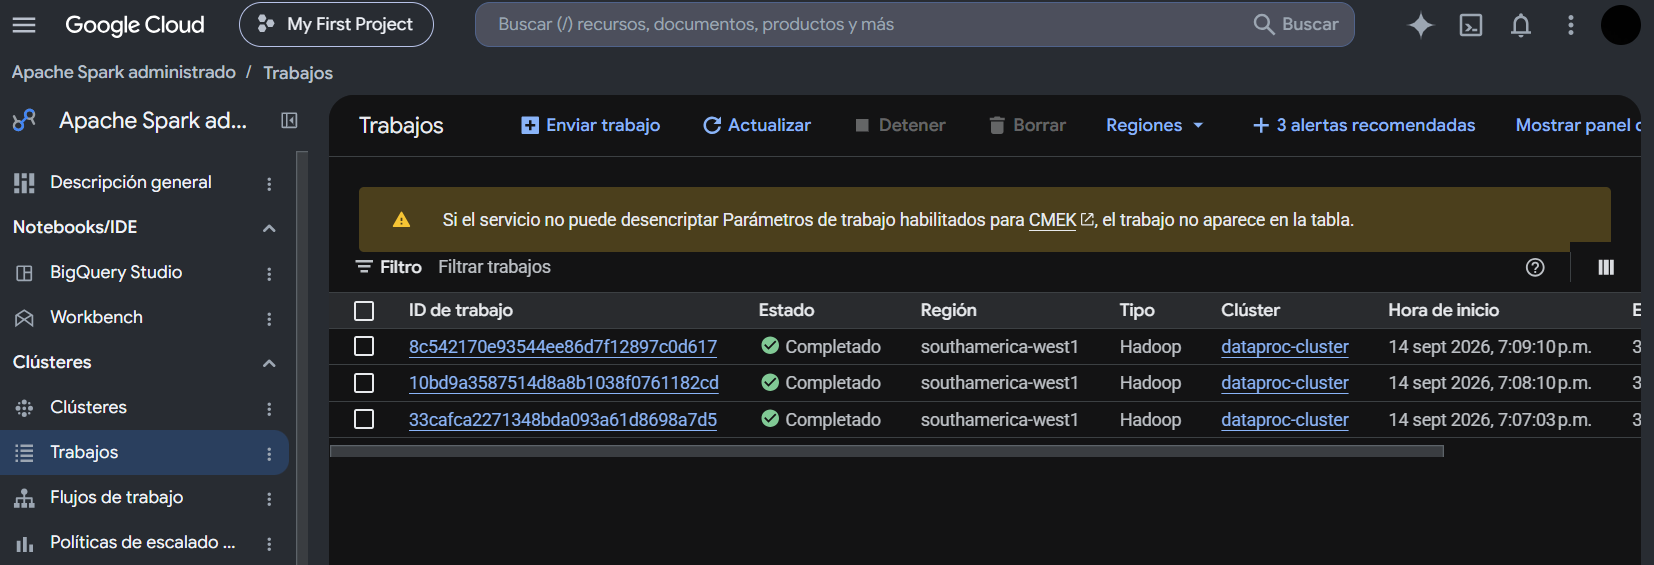
\includegraphics[width=0.9\textwidth]{../evidencia/dataproc-jobs-completados.png}
    \caption{Los tres jobs de Hadoop MapReduce en estado \emph{Completado}}
    \label{fig:dataproc-jobs}
\end{figure}

\textbf{\texttt{wordmean.txt}}: el programa no imprime la media directamente, sino los contadores con los que se calcula:

\begin{verbatim}
count   4664518
length  24485085
\end{verbatim}

Media = \texttt{length / count} $\approx$ 5.25 caracteres por palabra.

\textbf{\texttt{wordmedian.txt}}: a diferencia de \texttt{wordmean}, este programa sí entrega una tabla completa: para cada largo de palabra, cuántas palabras de ese largo aparecen en el catálogo. La Tabla \ref{tab:wordmedian} muestra el resultado completo, reordenado por largo (el archivo crudo sale desordenado porque el job usó 3 \emph{reducers} y cada uno escribió su propia partición).

\begin{table}[H]
\centering
\begin{tabular}{rrrr}
\toprule
\textbf{Largo} & \textbf{Palabras} & \textbf{Largo} & \textbf{Palabras} \\
\midrule
1 & 120{,}811 & 13 & 2{,}678 \\
2 & 216{,}503 & 14 & 664 \\
3 & 635{,}952 & 15 & 1{,}428 \\
4 & 832{,}710 & 16 & 1{,}273 \\
5 & 951{,}496 & 17 & 290 \\
6 & 666{,}273 & 18 & 377 \\
7 & 583{,}812 & 19 & 9 \\
8 & 272{,}244 & 20 & 23 \\
9 & 254{,}661 & 21 & 13 \\
10 & 88{,}601 & 22 & 144 \\
11 & 21{,}587 & 23 & 8 \\
12 & 12{,}961 & & \\
\bottomrule
\end{tabular}
\caption{Distribución real del largo de palabra en \texttt{descriptions.txt}, ordenada}
\label{tab:wordmedian}
\end{table}

Sumando estos conteos da exactamente 4{,}664{,}518 palabras, el mismo \texttt{count} de \texttt{wordmean.txt}, lo que confirma que ambos programas leyeron el mismo texto. La mitad de esa cantidad es 2{,}332{,}259: acumulando la tabla desde largo 1, se llega a 1{,}805{,}976 palabras hasta largo 4, y se pasa el 50\% recién al sumar el largo 5 (951{,}496 palabras más). Es decir, la mediana del largo de palabra es \textbf{5}, muy cerca de la media de 5.25 calculada arriba, y coincide con que largo 5 es también el bucket individual más grande de la tabla (casi 1 de cada 5 palabras del catálogo tiene 5 caracteres).

\textbf{\texttt{secondarysort.txt}}: compras agrupadas por \texttt{Customer ID} (5{,}942 clientes, el mismo total que en la Sección \ref{sec:dataset}), ordenadas ascendentemente por \texttt{Quantity} dentro de cada grupo (830{,}306 líneas, $\sim$7 MB). Más allá del ordenamiento en sí, esto deja ver el patrón de compra de cada cliente. Por ejemplo, el cliente \texttt{12348} tiene 51 líneas en el archivo, con estas cantidades distintas:

\begin{verbatim}
12348   1
12348   1
12348   1
12348   1
12348   6
12348   12
...
12348   24
...
12348   48
...
12348   72
...
12348   96
...
12348   120
...
12348   144
\end{verbatim}

De esas 51 compras, 44 (el 86\%) son múltiplos de 12, docenas, cuatro docenas, media gruesa, una gruesa, con solo 7 excepciones sueltas (cantidades de 1, 6, 20 y 80 unidades). Ese patrón dominante, comprar por docena y sus múltiplos, es consistente con un cliente mayorista (un negocio que revende, no una persona comprando para sí misma), en línea con lo ya señalado en la Sección \ref{sec:dataset}: el dataset está dominado por compras de otros negocios, no de consumidores finales. Las pocas compras sueltas podrían ser ajustes puntuales o pedidos de muestra, no cambian el patrón general. \texttt{secondarysort} permite ver esta clase de patrón por cliente sin tener que volver a leer el dataset completo, la agrupación y el orden secundario ya vienen resueltos por el propio job de MapReduce.

Estos tres resultados fueron reproducidos de forma independiente sobre un clúster Dataproc real, y los tres archivos completos están versionados en \url{hadoop-mapreduce/work/} del repositorio.
